% 图 51.6 —— 由 `checks/emit_hand.py` 自动拼出（probe 精测 + prims2 图元分解）
%%
% ⚠ 这是**稿子不是成品**：跑 `checks/checkhand.py 51.6` 看指标 + 看叠合图。
%%
%% ⚠ 待核：
%   · 本图 probe 报出阴影族 2 个 —— **本脚本不生成阴影**（要照原书手写）；prims2 的 strokes 里可能含阴影线，核对时留意别画重
%   · 可疑字形 3 项（空心圈 ⊙ 常被认成字母 o）—— 见文件末
%%
\documentclass[12pt]{standalone}
\usepackage{fontspec}
\setsansfont{Arial}
\newfontfamily\mfallback{DejaVu Sans}
\usepackage{tikz}
\begin{document}
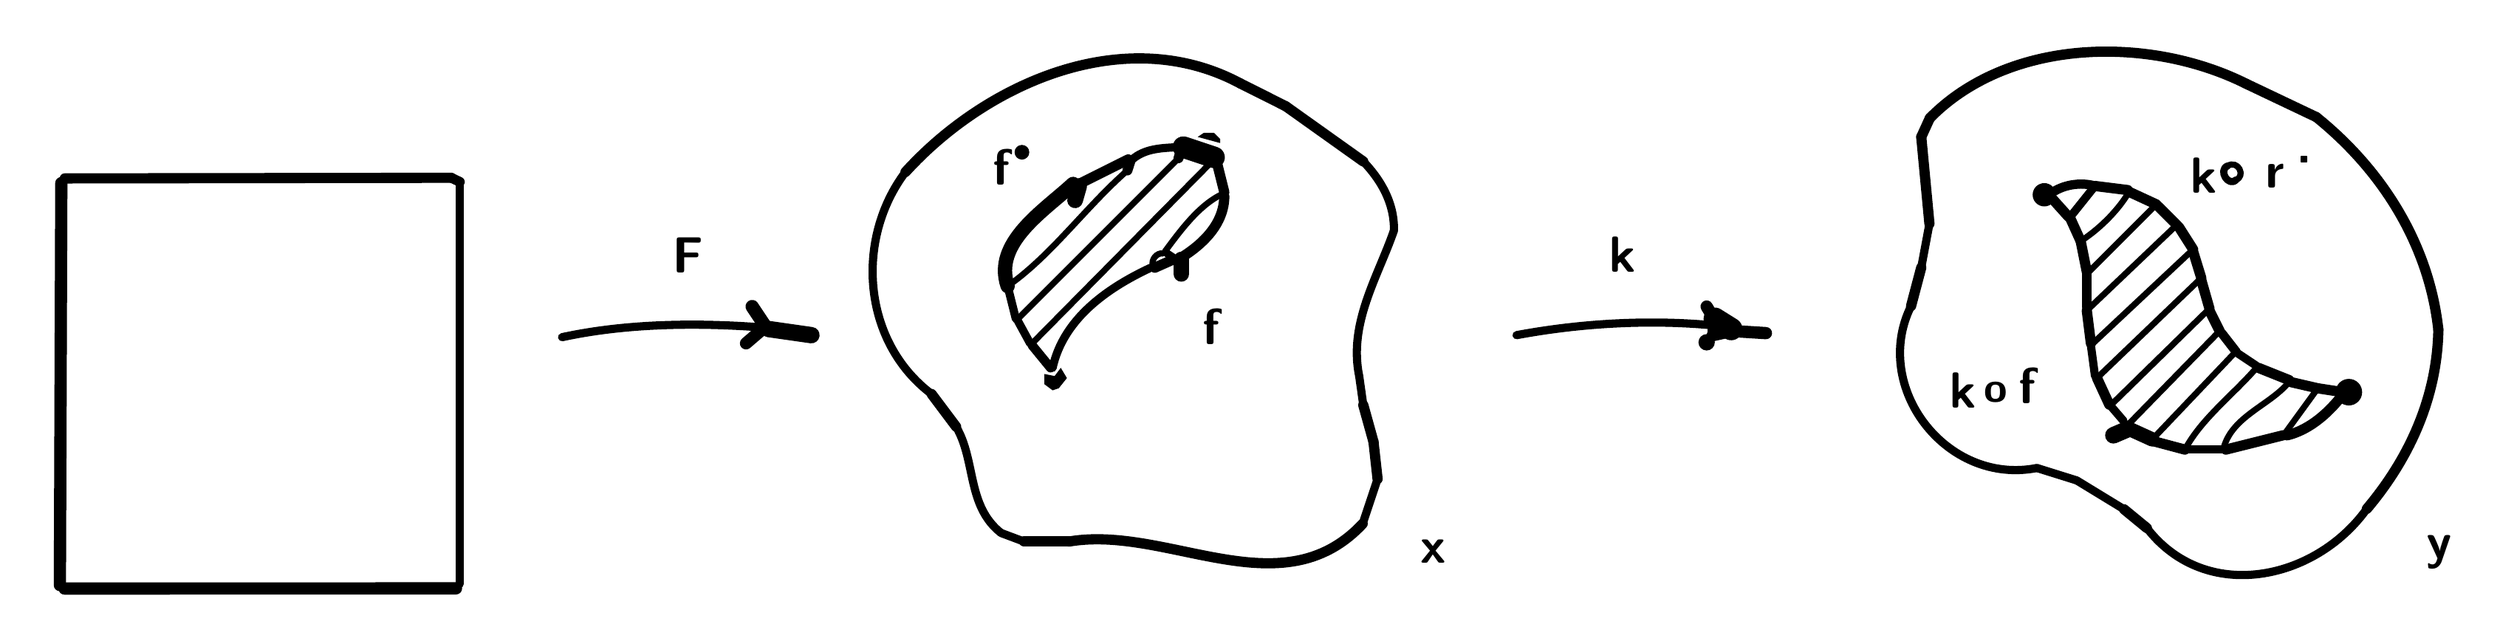
\begin{tikzpicture}[x=1pt, y=-1pt, line width=5.0pt, line cap=round, line join=round]

  %% ════ 填充区（prims2 的 fills）════
  \fill (576.0,57.0) -- (587.0,60.0) -- (587.0,58.0) -- (584.0,55.0) -- (579.0,55.0) -- cycle;
  \fill (509.0,170.0) -- (506.0,174.0) -- (501.0,173.0) -- (501.0,178.0) -- (505.0,181.0) -- (508.0,180.0) -- (512.0,175.0) -- cycle;

  %% ════ 直线段（prims2 的 strokes）════
  \draw[line width=5.0pt] (585.0,68.0) -- (589.0,84.0);
  \draw[line width=5.0pt] (993.0,86.0) -- (1002.0,96.0);
  \draw[line width=3.0pt] (1012.0,123.0) -- (1044.0,91.0);
  \draw[line width=5.0pt] (1111.0,177.0) -- (1124.0,180.0);
  \draw[line width=5.0pt] (1015.0,81.0) -- (1031.0,83.0);
  \draw[line width=4.0pt] (1015.0,81.0) -- (1003.0,96.0);
  \draw[line width=7.7pt] (568.0,124.0) -- (568.0,117.0);
  \draw[line width=3.8pt] (564.0,116.0) -- (561.0,114.0);
  \draw[line width=3.0pt] (1017.0,174.0) -- (1066.0,127.0);
  \draw[line width=5.0pt] (1016.0,175.0) -- (1022.0,188.0);
  \draw[line width=5.0pt] (1137.0,182.0) -- (1124.0,180.0);
  \draw[line width=4.9pt] (543.0,69.0) -- (541.6,73.4);
  \draw[line width=6.0pt] (828.0,145.0) -- (825.0,140.0);
  \draw[line width=4.0pt] (483.0,130.0) -- (487.0,146.0);
  \draw[line width=4.0pt] (1029.0,196.0) -- (1023.0,189.0);
  \draw[line width=3.0pt] (1124.0,180.0) -- (1108.0,202.0);
  \draw[line width=6.0pt] (355.0,158.0) -- (362.0,152.0);
  \draw[line width=5.0pt] (1107.0,203.0) -- (1079.0,210.0);
  \draw[line width=6.5pt] (358.0,140.0) -- (364.0,149.0);
  \draw[line width=11.0pt] (829.0,146.0) -- (837.0,151.0);
  \draw[line width=4.5pt] (1084.0,162.0) -- (1077.0,153.0);
  \draw[line width=7.0pt] (1043.0,205.0) -- (1032.0,200.0);
  \draw[line width=5.0pt] (555.0,121.0) -- (564.0,117.0);
  \draw[line width=10.5pt] (584.0,67.0) -- (569.0,62.0);
  \draw[line width=3.0pt] (1032.0,197.0) -- (1075.0,153.0);
  \draw[line width=8.1pt] (1031.0,200.0) -- (1024.0,203.0);
  \draw[line width=5.0pt] (1044.0,206.0) -- (1059.0,210.0);
  \draw[line width=8.0pt] (387.0,154.0) -- (366.0,151.0);
  \draw[line width=3.0pt] (362.0,152.0) -- (359.8,150.0);
  \draw[line width=5.0pt] (1011.0,124.0) -- (1011.0,140.0);
  \draw[line width=5.0pt] (1013.0,158.0) -- (1011.0,142.0);
  \draw[line width=3.0pt] (1023.0,188.0) -- (1070.0,142.0);
  \draw[line width=4.9pt] (568.0,63.0) -- (566.6,67.4);
  \draw[line width=3.0pt] (566.6,67.4) -- (488.0,146.0);
  \draw[line width=5.0pt] (1063.0,113.0) -- (1067.0,126.0);
  \draw[line width=4.0pt] (494.0,158.0) -- (488.0,147.0);
  \draw[line width=4.0pt] (1085.0,163.0) -- (1094.0,169.0);
  \draw[line width=4.0pt] (1059.0,210.0) -- (1077.0,210.0);
  \draw[line width=3.0pt] (827.0,153.0) -- (827.0,150.0);
  \draw[line width=6.0pt] (838.0,152.0) -- (854.0,153.0);
  \draw[line width=6.0pt] (837.0,152.0) -- (828.0,154.0);
  \draw[line width=5.0pt] (1032.0,84.0) -- (1045.0,90.0);
  \draw[line width=3.0pt] (1054.0,101.0) -- (1012.0,141.0);
  \draw[line width=3.0pt] (584.0,68.0) -- (495.0,158.0);
  \draw[line width=5.0pt] (1046.0,91.0) -- (1055.0,100.0);
  \draw[line width=5.0pt] (1056.0,101.0) -- (1063.0,112.0);
  \draw[line width=3.0pt] (1044.0,204.0) -- (1083.0,163.0);
  \draw[line width=5.0pt] (1110.0,176.0) -- (1095.0,170.0);
  \draw[line width=7.7pt] (518.0,81.0) -- (516.0,88.0);
  \draw[line width=5.0pt] (1071.0,142.0) -- (1076.0,152.0);
  \draw[line width=4.5pt] (495.0,159.0) -- (504.0,170.0);
  \draw[line width=5.0pt] (1011.0,123.0) -- (1008.0,108.0);
  \draw[line width=5.0pt] (1003.0,97.0) -- (1008.0,108.0);
  \draw[line width=5.0pt] (542.0,68.0) -- (518.0,80.0);
  \draw[line width=5.0pt] (1067.0,127.0) -- (1071.0,141.0);
  \draw[line width=3.0pt] (1062.0,113.0) -- (1014.0,158.0);
  \draw[line width=4.0pt] (1013.0,159.0) -- (1015.0,174.0);
  \draw[line width=5.0pt] (657.0,69.0) -- (619.1,42.0);
  \draw[line width=5.0pt] (619.1,42.0) -- (596.8,30.8);
  \draw[line width=5.0pt] (445.8,182.8) -- (457.8,198.8);
  \draw[line width=4.0pt] (479.8,250.8) -- (491.0,255.0);
  \draw[line width=5.0pt] (491.0,255.0) -- (513.0,255.0);
  \draw[line width=4.0pt] (656.7,246.3) -- (664.0,224.4);
  \draw[line width=5.0pt] (664.0,224.4) -- (662.0,206.2);
  \draw[line width=5.0pt] (662.0,206.2) -- (657.0,188.2);
  \draw[line width=4.0pt] (657.0,188.2) -- (655.0,174.0);
  \draw[line width=4.0pt] (215.0,115.0) -- (215.0,79.0);
  \draw[line width=4.8pt] (215.0,79.0) -- (210.8,77.0);
  \draw[line width=5.0pt] (210.8,77.0) -- (21.7,77.3);
  \draw[line width=2.9pt] (21.7,77.3) -- (20.0,79.6);
  \draw[line width=6.0pt] (20.0,79.6) -- (19.3,276.3);
  \draw[line width=2.9pt] (19.3,276.3) -- (21.6,278.0);
  \draw[line width=6.0pt] (21.6,278.0) -- (213.1,277.9);
  \draw[line width=2.9pt] (213.1,277.9) -- (215.0,275.7);
  \draw[line width=4.0pt] (215.0,275.7) -- (215.0,115.0);
  \draw[line width=5.0pt] (930.0,57.0) -- (934.2,47.8);
  \draw[line width=5.0pt] (1089.0,31.0) -- (1123.3,47.3);
  \draw[line width=5.0pt] (1040.4,248.4) -- (1029.2,239.2);
  \draw[line width=4.0pt] (1029.2,239.2) -- (1006.1,225.1);
  \draw[line width=4.0pt] (1006.1,225.1) -- (986.6,219.0);
  \draw[line width=5.0pt] (925.0,139.8) -- (930.0,120.9);
  \draw[line width=4.0pt] (930.0,120.9) -- (934.0,99.5);
  \draw[line width=5.0pt] (934.0,99.5) -- (930.0,57.0);

  %% ════ 曲线（prims2 的 curves —— 三段式，坐标同为 (y,x)）════
  \draw[line width=4.0pt] (505.0,170.0) .. controls (510.3,145.9) and (531.8,130.9) .. (553.0,121.0);
  \draw[line width=4.5pt] (1015.0,81.0) .. controls (1007.9,78.9) and (998.8,80.4) .. (993.0,85.0);
  \draw[line width=5.0pt] (1137.0,182.0) .. controls (1130.2,191.3) and (1120.3,200.3) .. (1109.0,203.0);
  \draw[line width=3.0pt] (541.6,73.4) .. controls (520.8,91.7) and (504.7,114.7) .. (483.0,130.0);
  \draw[line width=7.0pt] (483.0,130.0) .. controls (475.7,108.7) and (501.0,93.0) .. (515.0,80.0);
  \draw[line width=3.0pt] (559.0,114.0) .. controls (555.9,113.6) and (553.2,117.0) .. (554.0,120.0);
  \draw[line width=5.0pt] (568.0,116.0) .. controls (578.6,109.4) and (588.9,99.5) .. (589.0,86.0);
  \draw[line width=3.0pt] (560.0,113.0) .. controls (567.2,103.3) and (576.6,90.3) .. (588.0,85.0);
  \draw[line width=4.0pt] (359.8,150.0) .. controls (328.2,147.8) and (294.9,148.5) .. (265.0,155.0);
  \draw[line width=3.0pt] (1059.0,210.0) .. controls (1067.1,194.8) and (1082.7,183.1) .. (1094.0,170.0);
  \draw[line width=4.0pt] (567.0,62.0) .. controls (558.9,62.4) and (550.3,62.5) .. (544.0,68.0);
  \draw[line width=4.0pt] (732.0,154.0) .. controls (762.0,148.4) and (794.5,146.3) .. (826.0,149.0);
  \draw[line width=3.0pt] (1109.0,178.0) .. controls (1099.7,188.5) and (1082.2,194.0) .. (1078.0,209.0);
  \draw[line width=3.0pt] (1031.0,85.0) .. controls (1025.6,93.7) and (1016.8,102.3) .. (1008.0,108.0);
  \draw[line width=5.0pt] (596.8,30.8) .. controls (540.6,0.7) and (472.8,30.4) .. (433.0,74.2);
  \draw[line width=4.0pt] (433.0,74.2) .. controls (408.4,106.8) and (411.6,157.0) .. (445.8,182.8);
  \draw[line width=4.0pt] (457.8,198.8) .. controls (467.6,215.4) and (462.9,237.5) .. (479.8,250.8);
  \draw[line width=5.0pt] (513.0,255.0) .. controls (561.1,246.7) and (617.0,288.8) .. (656.7,246.3);
  \draw[line width=4.0pt] (655.0,174.0) .. controls (649.7,148.1) and (664.1,125.6) .. (672.0,102.8);
  \draw[line width=4.0pt] (672.0,102.8) .. controls (672.3,89.7) and (665.9,78.3) .. (657.0,69.0);
  \draw[line width=5.0pt] (934.2,47.8) .. controls (973.1,8.3) and (1041.9,7.4) .. (1089.0,31.0);
  \draw[line width=5.0pt] (1123.3,47.3) .. controls (1156.3,73.9) and (1178.5,110.3) .. (1183.0,151.4);
  \draw[line width=5.0pt] (1183.0,151.4) .. controls (1182.4,184.3) and (1169.0,214.1) .. (1148.0,239.0);
  \draw[line width=4.0pt] (1148.0,239.0) .. controls (1122.6,274.4) and (1069.0,285.4) .. (1040.4,248.4);
  \draw[line width=4.0pt] (986.6,219.0) .. controls (942.2,227.7) and (905.4,179.3) .. (925.0,139.8);
  \draw[line width=3.0pt] (1084.0,78.0) .. controls (1088.9,76.2) and (1085.1,68.0) .. (1079.8,71.2);
  \draw[line width=3.5pt] (1079.8,71.2) .. controls (1075.1,73.5) and (1080.4,81.6) .. (1084.0,78.0);

  %% ════ 实心点 ════
  \fill (490.0,64.5) circle (3.6);
  \fill (990.2,85.3) circle (5.7);
  \fill (825.0,157.5) circle (4.0);
  \fill (1139.2,181.9) circle (6.5);

  %% ════ 标签（probe 直接给的 \node 行）════
  %% ⚠ 全部补了 fill=white：文字在最上层，否则与曲线交叉干扰
     \node[anchor=center,inner sep=0pt,fill=white,font=\fontsize{29.1}{36.4}\selectfont] at (481.0,72.0) {\textsf{\textbf{\textit{f}}}};   % box(475,60,11,23)
     \node[anchor=center,inner sep=0pt,fill=white,font=\fontsize{30.1}{37.6}\selectfont] at (1068.3,76.0) {\textsf{\textbf{\textit{k}}}};   % box(1060,63,16,23)
     \node[anchor=center,inner sep=0pt,fill=white,font=\fontsize{39.0}{48.8}\selectfont] at (1103.3,76.3) {\textsf{\textbf{\textit{r}}}};   % box(1093,63,16,22)
     \node[anchor=center,inner sep=0pt,fill=white,font=\fontsize{50.3}{62.9}\selectfont] at (1117.3,67.9) {\textsf{\textbf{.}}};   % box(1111,63,5,9)
     \node[anchor=center,inner sep=0pt,fill=white,font=\fontsize{30.3}{37.9}\selectfont] at (783.8,114.5) {\textsf{\textbf{\textit{k}}}};   % box(775,102,17,22)
     \node[anchor=center,inner sep=0pt,fill=white,font=\fontsize{30.0}{37.4}\selectfont] at (326.5,115.0) {\textsf{\textbf{\textit{F}}}};   % box(317,103,19,22)
     \node[anchor=center,inner sep=0pt,fill=white,font=\fontsize{27.8}{34.7}\selectfont] at (583.5,150.0) {\textsf{\textbf{\textit{f}}}};   % box(578,138,10,23)
     \node[anchor=center,inner sep=0pt,fill=white,font=\fontsize{29.1}{36.4}\selectfont] at (983.0,179.0) {\textsf{\textbf{\textit{f}}}};   % box(977,167,11,23)
     \node[anchor=center,inner sep=0pt,fill=white,font=\fontsize{30.1}{37.6}\selectfont] at (950.3,181.0) {\textsf{\textbf{\textit{k}}}};   % box(942,168,16,23)
     \node[anchor=center,inner sep=0pt,fill=white,font=\fontsize{22.2}{27.7}\selectfont] at (966.6,182.1) {\textsf{\textbf{\textit{o}}}};   % box(960,175,12,12)
     \node[anchor=center,inner sep=0pt,fill=white,font=\fontsize{38.0}{47.5}\selectfont] at (691.3,260.0) {\textsf{\textbf{\textit{x}}}};   % box(680,246,20,23)
     \node[anchor=center,inner sep=0pt,fill=white,font=\fontsize{29.8}{37.3}\selectfont] at (1183.7,260.2) {\textsf{\textbf{\textit{y}}}};   % box(1175,247,17,23)

  % 钉死画布：否则超出的图元/控制点会把页面撑大，1:1 回比就失准
  \pgfresetboundingbox
  \path[use as bounding box] (0,0) rectangle (1203,285);
\end{tikzpicture}
\end{document}

% ⚠ 待核清单（probe 拿不准，人眼过一遍）：
%   · 可疑字形：\node[anchor=center,inner sep=0pt,font=\fontsize{22.2}{27.7}\selectfont] at (966.6,182.1) {\textsf{\textbf{\te
%   · 未识别/跳过：⑤ 跳过/未识别的字形
%   · 未识别/跳过：box(1078,70,11,12)
